\documentclass[11pt,letterpaper]{article}

% ============================================================================
% PACKAGES
% ============================================================================
\usepackage[utf8]{inputenc}
\usepackage[T1]{fontenc}
\usepackage{helvet}
\renewcommand{\familydefault}{\sfdefault}
\usepackage[margin=0.85in, headheight=28pt]{geometry}
\usepackage{graphicx}
\usepackage{xcolor}
\usepackage{tikz}
\usepackage{tcolorbox}
\usepackage{booktabs}
\usepackage{enumitem}
\usepackage{hyperref}
\usepackage{fancyhdr}
\usepackage{titlesec}
\usepackage{multicol}
\usepackage{listings}
\usepackage{upquote}
\usepackage{amsmath,amssymb}
\usepackage{pgfplots}
\usepackage{array}
\usepackage{longtable}
\usepackage{colortbl}
\usepackage{pifont}
\usepackage{setspace}
\usepackage{parskip}
\usepackage{caption}

\pgfplotsset{compat=1.18}
\usetikzlibrary{shapes.geometric, arrows.meta, positioning, calc, decorations.pathreplacing, backgrounds, fit, shadows.blur, matrix, patterns, fadings, shadings}

% ============================================================================
% COLOR DEFINITIONS - Modern AWS/Cloud Palette
% ============================================================================
\definecolor{awsdark}{HTML}{161E2D}         % Deep navy
\definecolor{awsblue}{HTML}{232F3E}         % AWS dark blue
\definecolor{awsorange}{HTML}{FF9900}       % AWS signature orange
\definecolor{awslightorange}{HTML}{FFAC33}  % Lighter orange
\definecolor{cloudblue}{HTML}{4A90D9}       % Sky blue
\definecolor{cloudlight}{HTML}{E8F4FD}      % Light cloud
\definecolor{successgreen}{HTML}{2ECC71}    % Success green
\definecolor{warningamber}{HTML}{F39C12}    % Warning amber
\definecolor{dangerred}{HTML}{E74C3C}       % Danger red
\definecolor{infoteal}{HTML}{17A2B8}        % Info teal
\definecolor{coolgray}{HTML}{6C757D}        % Cool gray
\definecolor{lightgray}{HTML}{F8F9FA}       % Light background
\definecolor{codebg}{HTML}{F7F7F7}          % Light code background
\definecolor{codetext}{HTML}{333333}        % Dark code text
\definecolor{codekeyword}{HTML}{0000FF}     % Blue keywords
\definecolor{codestring}{HTML}{008000}      % Green strings
\definecolor{codecomment}{HTML}{808080}     % Gray comments
\definecolor{codenumber}{HTML}{098658}      % Teal numbers
\definecolor{codeborder}{HTML}{E0E0E0}      % Border color

% ============================================================================
% HYPERREF SETUP
% ============================================================================
\hypersetup{
  colorlinks=true,
  linkcolor=cloudblue,
  urlcolor=awsorange,
  pdftitle={AWS Bedrock AgentCore Memory Integration Guide},
  pdfauthor={AI Agent Team}
}

% ============================================================================
% SPACING AND TYPOGRAPHY
% ============================================================================
\setstretch{1.15}
\setlength{\parskip}{0.5em}
\setlist{nosep, leftmargin=1.5em, itemsep=0.3em}

% ============================================================================
% PAGE STYLE
% ============================================================================
\pagestyle{fancy}
\fancyhf{}
\fancyhead[L]{%
  \begin{tikzpicture}[baseline=-0.5ex]
    \fill[awsorange] (0,0) circle (0.15);
    \fill[awsorange!70] (0.35,0) circle (0.1);
    \fill[awsorange!40] (0.6,0) circle (0.06);
  \end{tikzpicture}
  \hspace{0.3em}\textcolor{awsblue}{\textsf{\textbf{AgentCore Memory}}}%
}
\fancyhead[R]{\textcolor{coolgray}{\textsf{\thepage}}}
\fancyfoot[C]{\textcolor{coolgray}{\small\textsf{AWS Bedrock AgentCore Integration Guide}}}
\renewcommand{\headrulewidth}{0pt}
\renewcommand{\footrulewidth}{0pt}

% Add subtle top border
\fancyheadoffset{0pt}
\setlength{\headheight}{32pt}

% ============================================================================
% SECTION FORMATTING - Modern Style
% ============================================================================
\titleformat{\section}
  {\normalfont\LARGE\bfseries\color{awsblue}}
  {\colorbox{awsorange}{\textcolor{white}{\thesection}}}{0.8em}{}
\titleformat{\subsection}
  {\normalfont\Large\bfseries\color{awsblue!80}}
  {\thesubsection}{0.6em}{}
\titleformat{\subsubsection}
  {\normalfont\large\color{coolgray}\bfseries}
  {\thesubsubsection}{0.5em}{}

\titlespacing*{\section}{0pt}{3ex plus 1ex minus .2ex}{2ex plus .2ex}
\titlespacing*{\subsection}{0pt}{2.5ex plus 1ex minus .2ex}{1.5ex plus .2ex}

% ============================================================================
% TOC STYLING
% ============================================================================
\setcounter{tocdepth}{2}

% ============================================================================
% TCOLORBOX ENVIRONMENTS - Modern Redesign
% ============================================================================
\tcbuselibrary{skins,breakable,hooks}

% Key Concept Box - Gradient left border
\newtcolorbox{keybox}[1][Key Concept]{
  enhanced,
  breakable,
  colback=cloudlight,
  colframe=cloudblue,
  colbacktitle=cloudblue,
  coltitle=white,
  fonttitle=\bfseries\sffamily,
  title={\faLightbulb\hspace{0.5em}#1},
  boxrule=0pt,
  leftrule=4pt,
  arc=0pt,
  outer arc=0pt,
  left=12pt, right=12pt, top=8pt, bottom=8pt,
  shadow={2pt}{-2pt}{0pt}{black!20}
}

% Warning Box - Bold left accent
\newtcolorbox{warnbox}[1][Warning]{
  enhanced,
  breakable,
  colback=dangerred!5,
  colframe=dangerred,
  colbacktitle=dangerred,
  coltitle=white,
  fonttitle=\bfseries\sffamily,
  title={\faExclamationTriangle\hspace{0.5em}#1},
  boxrule=0pt,
  leftrule=4pt,
  arc=0pt,
  outer arc=0pt,
  left=12pt, right=12pt, top=8pt, bottom=8pt,
  shadow={2pt}{-2pt}{0pt}{black!15}
}

% Success/Tip Box
\newtcolorbox{tipbox}[1][Pro Tip]{
  enhanced,
  breakable,
  colback=successgreen!8,
  colframe=successgreen,
  colbacktitle=successgreen,
  coltitle=white,
  fonttitle=\bfseries\sffamily,
  title={\faCheckCircle\hspace{0.5em}#1},
  boxrule=0pt,
  leftrule=4pt,
  arc=0pt,
  outer arc=0pt,
  left=12pt, right=12pt, top=8pt, bottom=8pt,
  shadow={2pt}{-2pt}{0pt}{black!15}
}

% AWS Service Box - Orange accent
\newtcolorbox{awsbox}[1][AWS Service]{
  enhanced,
  breakable,
  colback=awsorange!5,
  colframe=awsorange,
  colbacktitle=awsorange,
  coltitle=white,
  fonttitle=\bfseries\sffamily,
  title={\faAws\hspace{0.5em}#1},
  boxrule=0pt,
  leftrule=4pt,
  arc=0pt,
  outer arc=0pt,
  left=12pt, right=12pt, top=8pt, bottom=8pt,
  shadow={2pt}{-2pt}{0pt}{black!15}
}

% Info Box - Teal accent
\newtcolorbox{infobox}[1][Note]{
  enhanced,
  breakable,
  colback=infoteal!5,
  colframe=infoteal,
  colbacktitle=infoteal,
  coltitle=white,
  fonttitle=\bfseries\sffamily,
  title={\faInfoCircle\hspace{0.5em}#1},
  boxrule=0pt,
  leftrule=4pt,
  arc=0pt,
  outer arc=0pt,
  left=12pt, right=12pt, top=8pt, bottom=8pt,
  shadow={2pt}{-2pt}{0pt}{black!15}
}

% TL;DR Summary Box - Prominent
\newtcolorbox{tldrbox}{
  enhanced,
  breakable,
  colback=awsblue!3,
  colframe=awsblue,
  boxrule=1.5pt,
  arc=8pt,
  outer arc=8pt,
  left=15pt, right=15pt, top=12pt, bottom=12pt,
  fontupper=\small,
  before upper={\textcolor{awsorange}{\faRocket}\hspace{0.5em}\textbf{TL;DR}\hspace{0.8em}},
  shadow={3pt}{-3pt}{0pt}{black!20}
}

% ============================================================================
% CODE LISTING STYLE - Light Theme for Readability
% ============================================================================
\lstdefinestyle{moderncode}{
  language=Python,
  basicstyle=\ttfamily\small\color{codetext},
  keywordstyle=\color{codekeyword}\bfseries,
  stringstyle=\color{codestring},
  commentstyle=\color{codecomment}\itshape,
  backgroundcolor=\color{codebg},
  frame=single,
  rulecolor=\color{codeborder},
  framesep=8pt,
  numbers=left,
  numberstyle=\tiny\color{coolgray},
  numbersep=12pt,
  breaklines=true,
  showstringspaces=false,
  tabsize=4,
  xleftmargin=25pt,
  framexleftmargin=20pt,
  aboveskip=1em,
  belowskip=1em,
  literate={`}{\`}1
}
\lstset{style=moderncode}

% Custom caption format for listings
\DeclareCaptionFormat{codecaption}{%
  \begin{tcolorbox}[
    enhanced,
    colback=awsblue!5,
    colframe=awsblue!50,
    boxrule=0.5pt,
    arc=4pt,
    left=8pt, right=8pt, top=4pt, bottom=4pt,
    before skip=0pt,
    after skip=0.5em
  ]
  \textcolor{awsblue}{\faFileCode}\hspace{0.5em}\small\sffamily #1#2#3
  \end{tcolorbox}
}
\captionsetup[lstlisting]{format=codecaption, labelfont={bf}, textfont={}, skip=0pt}

% ============================================================================
% ICON COMMANDS (pifont replacements for fontawesome5)
% ============================================================================
\newcommand{\faRobot}{\ding{70}}
\newcommand{\faCheck}{\ding{51}}
\newcommand{\faCheckCircle}{\ding{51}}
\newcommand{\faTimes}{\ding{55}}
\newcommand{\faTimesCircle}{\ding{55}}
\newcommand{\faExclamationTriangle}{\ding{74}}
\newcommand{\faExclamationCircle}{\ding{74}}
\newcommand{\faLightbulb}{\ding{72}}
\newcommand{\faInfoCircle}{\ding{73}}
\newcommand{\faRocket}{\ding{228}}
\newcommand{\faDatabase}{\ding{115}}
\newcommand{\faTachometerAlt}{\ding{99}}
\newcommand{\faAws}{\textbf{AWS}}
\newcommand{\faCloud}{\ding{110}}
\newcommand{\faBrain}{\ding{70}}
\newcommand{\faServer}{\ding{115}}
\newcommand{\faProjectDiagram}{\ding{118}}
\newcommand{\faLayerGroup}{\ding{115}}
\newcommand{\faCode}{\texttt{</>}}
\newcommand{\faCogs}{\ding{70}}
\newcommand{\faShieldAlt}{\ding{110}}
\newcommand{\faKey}{\ding{70}}
\newcommand{\faEye}{\ding{70}}
\newcommand{\faCloudUploadAlt}{\ding{110}}
\newcommand{\faChartLine}{\ding{70}}
\newcommand{\faDollarSign}{\$}
\newcommand{\faBook}{\ding{70}}
\newcommand{\faFileCode}{\ding{70}}
\newcommand{\faPython}{\ding{70}}
\newcommand{\faGithub}{\ding{70}}
\newcommand{\faListAlt}{\ding{70}}
\newcommand{\faClock}{\ding{70}}
\newcommand{\faSearch}{\ding{70}}
\newcommand{\faCog}{\ding{70}}
\newcommand{\faSquare}{\ding{111}}
\newcommand{\faCalculator}{\ding{70}}
\newcommand{\faBan}{\ding{55}}
\newcommand{\faFileAlt}{\ding{70}}
\newcommand{\faRandom}{\ding{70}}
\newcommand{\faEraser}{\ding{70}}
\newcommand{\faLock}{\ding{70}}
\newcommand{\faUserShield}{\ding{70}}

% ============================================================================
% CUSTOM COMMANDS
% ============================================================================
\newcommand{\api}[1]{\texttt{\textcolor{cloudblue}{#1}}}
\newcommand{\code}[1]{\texttt{\small\colorbox{lightgray}{#1}}}
\newcommand{\ratelimit}{\textcolor{dangerred}{\faExclamationCircle\ 0.25 req/sec}}

% ============================================================================
% PART PAGE STYLING
% ============================================================================
\newcommand{\partpage}[4]{%
  \clearpage
  \thispagestyle{empty}
  \begin{tikzpicture}[remember picture, overlay]
    % Gradient background
    \shade[top color=awsdark, bottom color=awsblue]
      (current page.north west) rectangle ([yshift=-9cm]current page.north east);

    % Decorative circles
    \fill[awsorange, opacity=0.15] ([xshift=12cm, yshift=-3cm]current page.north west) circle (4cm);
    \fill[awsorange, opacity=0.1] ([xshift=14cm, yshift=-6cm]current page.north west) circle (2.5cm);
    \fill[cloudblue, opacity=0.1] ([xshift=3cm, yshift=-5cm]current page.north west) circle (3cm);

    % Part number - large and prominent
    \node[white, opacity=0.08, font=\fontsize{200}{200}\selectfont\bfseries]
      at ([xshift=5cm, yshift=-5cm]current page.north west) {#1};

    % Part label
    \node[white, font=\large\sffamily] at ([yshift=-2.5cm]current page.north) {PART};

    % Part number (visible)
    \node[awsorange, font=\fontsize{72}{72}\selectfont\bfseries]
      at ([yshift=-4.5cm]current page.north) {#1};

    % Part title
    \node[white, font=\Huge\bfseries\sffamily] at ([yshift=-7cm]current page.north) {#2};

    % Decorative line
    \draw[awsorange, line width=2pt]
      ([xshift=5cm, yshift=-8cm]current page.north west) --
      ([xshift=-5cm, yshift=-8cm]current page.north east);
  \end{tikzpicture}

  \vspace{9.5cm}

  % Overview content
  \begin{center}
  \begin{minipage}{0.88\textwidth}
    \begin{tcolorbox}[
      enhanced,
      colback=white,
      colframe=awsorange!50,
      boxrule=1pt,
      arc=6pt,
      left=15pt, right=15pt, top=12pt, bottom=12pt,
      shadow={2pt}{-2pt}{0pt}{black!15}
    ]
    \textcolor{awsblue}{\faListAlt\hspace{0.5em}\textbf{What's Covered}}
    \vspace{0.5em}

    #3
    \end{tcolorbox}

    \vspace{1em}

    % Icon row
    \begin{center}
    #4
    \end{center}
  \end{minipage}
  \end{center}
}

% ============================================================================
% DOCUMENT
% ============================================================================
\begin{document}

% ============================================================================
% TITLE PAGE - Full Page Design with remember picture
% ============================================================================
\begin{titlepage}

\begin{tikzpicture}[remember picture, overlay]
  % Left panel gradient (full height)
  \shade[left color=awsdark, right color=awsblue!90]
    (current page.north west) rectangle ([xshift=7cm]current page.south west);

  % Decorative circles on left panel
  \fill[awsorange, opacity=0.15] ([xshift=3.5cm, yshift=-4cm]current page.north west) circle (1.2cm);
  \fill[awsorange, opacity=0.10] ([xshift=3.5cm, yshift=-8cm]current page.north west) circle (0.9cm);
  \fill[cloudblue, opacity=0.12] ([xshift=3.5cm, yshift=-12cm]current page.north west) circle (1.1cm);
  \fill[awsorange, opacity=0.08] ([xshift=3.5cm, yshift=-16cm]current page.north west) circle (1.4cm);
  \fill[cloudblue, opacity=0.10] ([xshift=3.5cm, yshift=-20cm]current page.north west) circle (0.8cm);

  % Memory hub visualization centered at left panel
  \begin{scope}[shift={([xshift=3.5cm, yshift=-14cm]current page.north west)}]
    % Glow rings
    \fill[awsorange, opacity=0.08] (0,0) circle (2.8cm);
    \fill[awsorange, opacity=0.12] (0,0) circle (2.2cm);

    % Central hub
    \fill[awsorange] (0,0) circle (0.65cm);
    \node[white, font=\small\bfseries] at (0,0) {MEM};

    % Agent nodes around hub
    \foreach \angle/\label/\col in {60/C/cloudblue, 120/G/successgreen, 180/O/infoteal, 240/X/warningamber, 300/R/dangerred, 0/P/coolgray} {
      \draw[white, opacity=0.4, line width=1.5pt] (0,0) -- (\angle:1.6cm);
      \fill[\col] (\angle:2cm) circle (0.35cm);
      \node[white, font=\tiny\bfseries] at (\angle:2cm) {\label};
    }

    % Data particles
    \foreach \i in {1,...,12} {
      \fill[white, opacity=0.5] ({30*\i}:1cm) circle (0.05cm);
    }
  \end{scope}

  % ========== RIGHT SIDE CONTENT ==========

  % AWS Badge
  \node[fill=awsorange, rounded corners=3pt, inner sep=6pt]
    at ([xshift=11cm, yshift=-3cm]current page.north west)
    {\textcolor{white}{\small\bfseries\sffamily AWS BEDROCK}};

  % Main Title
  \node[anchor=west] at ([xshift=8cm, yshift=-5.5cm]current page.north west) {
    {\fontsize{48}{54}\selectfont\bfseries\color{awsblue}AgentCore}
  };
  \node[anchor=west] at ([xshift=8cm, yshift=-7.5cm]current page.north west) {
    {\fontsize{38}{44}\selectfont\color{cloudblue}Memory}
  };
  \node[anchor=west] at ([xshift=8cm, yshift=-9cm]current page.north west) {
    {\Large\color{coolgray}\sffamily Integration Guide}
  };

  % Tagline
  \node[anchor=west] at ([xshift=8cm, yshift=-11cm]current page.north west) {
    {\large\color{awsblue}\sffamily Persistent Memory for AI Agent Ecosystems}
  };

  % Orange divider
  \draw[awsorange, line width=3pt]
    ([xshift=8cm, yshift=-12cm]current page.north west) --
    ([xshift=18cm, yshift=-12cm]current page.north west);

  % Description
  \node[anchor=north west, text width=10cm] at ([xshift=8cm, yshift=-13cm]current page.north west) {
    \color{coolgray}\normalsize
    Enable your AI agents to remember context across sessions, share knowledge,
    and leverage semantic search---all backed by AWS managed infrastructure.
  };

  % Feature highlights
  \node[fill=cloudblue!10, rounded corners=4pt, inner sep=8pt]
    at ([xshift=9.5cm, yshift=-16.5cm]current page.north west) {
    \textcolor{cloudblue}{\faBrain}\hspace{0.3em}\small\sffamily Short-Term Events
  };
  \node[fill=successgreen!10, rounded corners=4pt, inner sep=8pt]
    at ([xshift=13.5cm, yshift=-16.5cm]current page.north west) {
    \textcolor{successgreen}{\faDatabase}\hspace{0.3em}\small\sffamily Long-Term Facts
  };
  \node[fill=awsorange!10, rounded corners=4pt, inner sep=8pt]
    at ([xshift=17.5cm, yshift=-16.5cm]current page.north west) {
    \textcolor{awsorange}{\faSearch}\hspace{0.3em}\small\sffamily Semantic Search
  };

  % Rate limit indicators
  \node[fill=dangerred!10, rounded corners=3pt, inner sep=6pt]
    at ([xshift=10cm, yshift=-19cm]current page.north west) {
    \textcolor{dangerred}{\faTimes}\hspace{0.3em}\scriptsize\sffamily Rate Limited
  };
  \node[fill=successgreen!10, rounded corners=3pt, inner sep=6pt]
    at ([xshift=14cm, yshift=-19cm]current page.north west) {
    \textcolor{successgreen}{\faCheck}\hspace{0.3em}\scriptsize\sffamily No Limit
  };

  % Version info
  \node[coolgray, font=\sffamily] at ([xshift=13cm, yshift=-21cm]current page.north west) {
    Version 1.0 | December 4, 2025
  };
\end{tikzpicture}
\end{titlepage}

% ============================================================================
% EXECUTIVE SUMMARY
% ============================================================================
\newpage
\thispagestyle{empty}

\begin{center}
{\color{awsblue}\fontsize{28}{32}\selectfont\bfseries Executive Summary}
\end{center}

\vspace{1cm}

\begin{tldrbox}
AI agents are stateless. This integration adds persistent memory via AWS Bedrock AgentCore,
enabling cross-session context and shared knowledge across your entire agent ecosystem.
\end{tldrbox}

\vspace{1.5em}

% Enhanced Problem/Solution/Constraint cards with side icons
\begin{tikzpicture}
  \node[fill=dangerred!8, rounded corners=10pt, text width=0.88\textwidth, inner sep=15pt, anchor=north west,
        drop shadow={shadow xshift=2pt, shadow yshift=-2pt, opacity=0.15}] (prob) at (1.2,0) {
    \textcolor{dangerred}{\textbf{THE PROBLEM}}\\[0.5em]
    \color{awsblue}AI agents (Claude Code, Gemini, OpenCode, Crush, Codex) lose all context between sessions.
    Each conversation starts from scratch---no memory of codebase patterns, user preferences, or prior learnings.
  };
  % Side icon
  \node[fill=dangerred, circle, minimum size=1cm, inner sep=0pt] at (0.4, -0.7) {
    \textcolor{white}{\large\faBrain}
  };
\end{tikzpicture}

\vspace{0.8em}

\begin{tikzpicture}
  \node[fill=successgreen!8, rounded corners=10pt, text width=0.88\textwidth, inner sep=15pt, anchor=north west,
        drop shadow={shadow xshift=2pt, shadow yshift=-2pt, opacity=0.15}] at (1.2,0) {
    \textcolor{successgreen}{\textbf{THE SOLUTION}}\\[0.5em]
    \color{awsblue}AWS Bedrock AgentCore Memory provides managed short-term and long-term memory.
    A new MCP server bridges your local agents with cloud-based persistent storage.
  };
  % Side icon
  \node[fill=successgreen, circle, minimum size=1cm, inner sep=0pt] at (0.4, -0.7) {
    \textcolor{white}{\large\faCloud}
  };
\end{tikzpicture}

\vspace{0.8em}

\begin{tikzpicture}
  \node[fill=awsorange!8, rounded corners=10pt, text width=0.88\textwidth, inner sep=15pt, anchor=north west,
        drop shadow={shadow xshift=2pt, shadow yshift=-2pt, opacity=0.15}] at (1.2,0) {
    \textcolor{awsorange}{\textbf{KEY CONSTRAINT}}\\[0.5em]
    \color{awsblue}The \api{CreateEvent} API is rate-limited to \textbf{0.25 req/sec per actor+session}.
    This is NOT a logging system---use it for sparse, high-value events only.
    Long-term facts via \api{BatchCreateMemoryRecords} have no such limit.
  };
  % Side icon
  \node[fill=awsorange, circle, minimum size=1cm, inner sep=0pt] at (0.4, -0.7) {
    \textcolor{white}{\large\faTachometerAlt}
  };
\end{tikzpicture}

\vspace{1.5em}

% API Overview Table
\begin{center}
\renewcommand{\arraystretch}{1.4}
\begin{tabular}{>{\raggedright}p{3.5cm} >{\centering}p{5cm} >{\raggedright\arraybackslash}p{5.5cm}}
\rowcolor{awsblue!10}
\textbf{\color{awsblue}Memory Type} & \textbf{\color{awsblue}API} & \textbf{\color{awsblue}Use Case} \\
\midrule
Short-term events & \api{CreateEvent} \textcolor{dangerred}{\tiny(0.25/s)} & Session goals, key decisions \\
Long-term facts & \api{BatchCreateMemoryRecords} & Patterns, preferences, learnings \\
Semantic search & \api{RetrieveMemoryRecords} & Context retrieval by meaning \\
\bottomrule
\end{tabular}
\end{center}

\vspace{2em}

% Architecture Preview
\begin{center}
\begin{tikzpicture}[
  layer/.style={rectangle, rounded corners=6pt, minimum height=1.2cm, font=\small\sffamily},
  arrow/.style={->, thick, >=stealth, awsblue!70}
]
  % Agents layer
  \node[layer, fill=cloudlight, draw=cloudblue, minimum width=12cm] (agents) at (0,2) {
    \faRobot\ \ Claude \quad\faRobot\ \ Gemini \quad\faRobot\ \ OpenCode \quad\faRobot\ \ Crush \quad\faRobot\ \ Codex
  };

  % MCP layer
  \node[layer, fill=awsblue!10, draw=awsblue, minimum width=12cm] (mcp) at (0,0) {
    \textbf{mcp-agentcore-memory} \textcolor{coolgray}{(aiobotocore)}
  };

  % AWS layer
  \node[layer, fill=awsorange!10, draw=awsorange, minimum width=12cm] (aws) at (0,-2) {
    \faAws\ \ AWS Bedrock AgentCore Memory
  };

  \draw[arrow] (agents) -- (mcp);
  \draw[arrow, awsorange] (mcp) -- node[right, font=\tiny, color=coolgray] {HTTPS} (aws);

  % Labels
  \node[coolgray, font=\tiny, anchor=east] at ([xshift=-0.5cm]agents.west) {Self-Hosted};
  \node[coolgray, font=\tiny, anchor=east] at ([xshift=-0.5cm]aws.west) {AWS Cloud};
\end{tikzpicture}
\end{center}

% ============================================================================
% TABLE OF CONTENTS
% ============================================================================
\newpage
\tableofcontents
\newpage

% ============================================================================
% CRITICAL CORRECTIONS FROM EXTERNAL REVIEWS
% ============================================================================
\section*{\faExclamationTriangle\ Critical Corrections from External Reviews}
\addcontentsline{toc}{section}{Critical Corrections}

\begin{warnbox}[This Section Documents Breaking Changes!]
Two external reviews identified critical issues that \textbf{fundamentally changed} the implementation approach. Review this section before implementing.
\end{warnbox}

\vspace{1em}

\subsection*{First Review: Hard Blockers}

\begin{center}
\renewcommand{\arraystretch}{1.5}
\begin{tabular}{>{\raggedright}p{3cm} >{\raggedright}p{4.5cm} >{\raggedright\arraybackslash}p{6cm}}
\rowcolor{dangerred!15}
\textbf{\color{dangerred}Issue} & \textbf{\color{dangerred}Impact} & \textbf{\color{dangerred}Resolution} \\
\midrule
\rowcolor{lightgray}
Rate limits wrong & CreateEvent is 0.25 req/sec per actor+session (not 100 TPS). ``Store every turn'' will throttle immediately. & Store coarse-grained events only; use BatchCreateMemoryRecords for facts \\
Control vs Data plane & CreateMemory is control plane, events are data plane. PrivateLink doesn't cover control plane. & Use separate clients; accept control plane uses public endpoint \\
\rowcolor{lightgray}
API shapes wrong & Response paths, payload formats don't match actual AWS APIs & Rewrite client to match actual API docs \\
async + boto3 = blocking & boto3 is synchronous; will stall MCP server under load & Use aiobotocore/aioboto3 for truly async calls \\
\bottomrule
\end{tabular}
\end{center}

\vspace{1.5em}

\subsection*{Second Review: Implementation Fixes}

\begin{center}
\renewcommand{\arraystretch}{1.5}
\begin{tabular}{>{\raggedright}p{3.5cm} >{\raggedright}p{4cm} >{\raggedright\arraybackslash}p{6cm}}
\rowcolor{warningamber!15}
\textbf{\color{warningamber}Issue} & \textbf{\color{warningamber}Impact} & \textbf{\color{warningamber}Resolution} \\
\midrule
\rowcolor{lightgray}
CreateEvent payload shape & Code will 400---branchName (string) vs branch (struct) & Fixed: \code{branch=\{"name": ...\}}, payload as list of unions \\
RetrieveMemoryRecords query & API requires searchQuery; empty fails & Fixed: query parameter now required; added separate list method \\
\rowcolor{lightgray}
Rate limiter not keyed & Global limiter doesn't match per-session limit & Fixed: \code{PerSessionRateLimiter} keyed by (actor\_id, session\_id) \\
Restore uses CreateEvent & Would take forever at 0.25/s & Fixed: Use BatchCreateMemoryRecords for restore \\
\rowcolor{lightgray}
Tests mock boto3 & Implementation uses aiobotocore; tests give false confidence & Fixed: Mock \code{\_get\_data\_plane\_client} with AsyncMock \\
Sanitize patterns incomplete & Missing AWS keys, GitHub tokens & Fixed: Added AKIA pattern, gh[pousr]\_ pattern, entropy detection \\
\bottomrule
\end{tabular}
\end{center}

\vspace{1.5em}

\subsection*{Third Review: Real AWS Integration Testing (2025-12)}

\begin{center}
\renewcommand{\arraystretch}{1.5}
\begin{tabular}{>{\raggedright}p{3.8cm} >{\raggedright}p{4cm} >{\raggedright\arraybackslash}p{5.7cm}}
\rowcolor{successgreen!15}
\textbf{\color{successgreen}Issue} & \textbf{\color{successgreen}Impact} & \textbf{\color{successgreen}Resolution} \\
\midrule
\rowcolor{lightgray}
BatchCreate param name & API expects \code{records}, not \code{memoryRecords} & Fixed: Changed parameter name \\
BatchCreate record structure & Requires \code{requestIdentifier}, \code{namespaces} (list), \code{timestamp} & Fixed: Added all required fields \\
\rowcolor{lightgray}
BatchCreate response shape & Returns \code{successfulRecords}/\code{failedRecords}, not \code{memoryRecords}/\code{errors} & Fixed: Updated response parsing \\
RetrieveRecords searchCriteria & Uses \code{searchQuery} (string), not \code{semanticQuery} (struct) & Fixed: Changed to simple string \\
\rowcolor{lightgray}
eventExpiryDuration units & Value is in DAYS (max 365), not ISO 8601 duration & Fixed: Changed to integer days \\
Memory name constraints & Must match \code{[a-zA-Z][a-zA-Z0-9\_]\{0,47\}} (no dashes!) & Fixed in setup script \\
\bottomrule
\end{tabular}
\end{center}

\vspace{1.5em}

\subsection*{Design Philosophy Changes}

\begin{center}
\begin{tikzpicture}[
  box/.style={rectangle, rounded corners=8pt, minimum width=6.5cm, minimum height=2.5cm,
    font=\small\sffamily, align=left, text width=6cm, inner sep=10pt}
]
  % Original design (crossed out)
  \node[box, fill=dangerred!10, draw=dangerred] (orig) at (-4, 0) {
    \textbf{\color{dangerred}\faTimes\ Original (Wrong)}\\[0.5em]
    \textcolor{coolgray}{\textbullet\ \code{store\_event} for every turn}\\
    \textcolor{coolgray}{\textbullet\ 100 TPS assumption}\\
    \textcolor{coolgray}{\textbullet\ ``100 MB = \$0.50'' pricing}\\
    \textcolor{coolgray}{\textbullet\ PrivateLink everywhere}
  };

  % Corrected design
  \node[box, fill=successgreen!10, draw=successgreen] (corr) at (4, 0) {
    \textbf{\color{successgreen}\faCheck\ Corrected}\\[0.5em]
    \textcolor{awsblue}{\textbullet\ Sparse events: goals, decisions, outcomes}\\
    \textcolor{awsblue}{\textbullet\ 0.25 req/sec per actor+session}\\
    \textcolor{awsblue}{\textbullet\ Per-record/day pricing}\\
    \textcolor{awsblue}{\textbullet\ PrivateLink = data plane only (+ VPC)}
  };

  % Arrow
  \draw[->, very thick, awsorange, >=stealth] (orig) -- (corr);
\end{tikzpicture}
\end{center}

\newpage

% ============================================================================
% PART I: ARCHITECTURE
% ============================================================================
\partpage{I}{Architecture}{%
\begin{itemize}[leftmargin=1.5em]
  \item \textbf{Section 1:} Current state analysis---why agents forget everything
  \item \textbf{Section 2:} Proposed architecture with AWS AgentCore integration
  \item \textbf{Section 3:} Multi-provider abstraction for flexibility
\end{itemize}
}{%
\textcolor{cloudblue}{\faProjectDiagram}\quad
\textcolor{awsorange}{\faAws}\quad
\textcolor{successgreen}{\faLayerGroup}
}

\section{Current State Analysis}

\begin{tldrbox}
All agents are stateless. No memory persists. Agents can't share knowledge. This limits effectiveness on long-running projects.
\end{tldrbox}

\subsection{The Stateless Agent Problem}

\begin{keybox}[Core Problem]
Current AI agents operate in \textbf{isolated sessions}:
\begin{itemize}
  \item Each session starts with zero context about the codebase
  \item Learnings from PR reviews vanish after the review ends
  \item User preferences must be re-established every time
  \item Agents cannot benefit from each other's discoveries
\end{itemize}
\end{keybox}

\vspace{1em}

% Visual diagram of the problem
\begin{center}
\begin{tikzpicture}[
  agent/.style={rectangle, rounded corners=8pt, fill=cloudlight, draw=cloudblue,
    minimum width=2.8cm, minimum height=1.2cm, font=\small\bfseries\sffamily},
  mcp/.style={rectangle, rounded corners=6pt, fill=awsblue!8, draw=awsblue!50,
    minimum width=10cm, minimum height=1cm, font=\small\sffamily},
  problem/.style={rectangle, rounded corners=8pt, fill=dangerred!10, draw=dangerred,
    text width=8cm, align=center, inner sep=10pt, font=\small},
  arrow/.style={->, thick, cloudblue!70, >=stealth}
]
  % Agents
  \node[agent] (claude) at (0, 2.5) {\faRobot\ Claude};
  \node[agent] (gemini) at (4, 2.5) {\faRobot\ Gemini};
  \node[agent] (opencode) at (8, 2.5) {\faRobot\ OpenCode};

  % MCP layer
  \node[mcp] (mcp) at (4, 0.5) {MCP Servers (code-quality, github-board, ...)};

  % Arrows
  \draw[arrow] (claude) -- (mcp);
  \draw[arrow] (gemini) -- (mcp);
  \draw[arrow] (opencode) -- (mcp);

  % Problem callout
  \node[problem] at (4, -1.8) {
    \textcolor{dangerred}{\faTimesCircle}\quad\textbf{No persistent memory layer!}\\[0.3em]
    Agents forget everything between sessions.
  };

  % Dashed line showing gap
  \draw[dashed, dangerred, thick] (0, -0.5) -- (8, -0.5);
\end{tikzpicture}
\end{center}

\subsection{Goals and Non-Goals}

\begin{multicols}{2}
\begin{tipbox}[Goals]
\begin{itemize}
  \item Cross-session memory for all agents
  \item Shared knowledge base
  \item Semantic search for retrieval
  \item Enterprise-ready AWS backend
\end{itemize}
\end{tipbox}

\columnbreak

\begin{warnbox}[Non-Goals]
\begin{itemize}
  \item Replace GitHub Board for coordination
  \item Migrate agents to AWS cloud
  \item Auto-inject context (explicit only)
  \item \textcolor{dangerred}{Log every conversation turn!}
\end{itemize}
\end{warnbox}
\end{multicols}

\section{Proposed Architecture}

\begin{tldrbox}
New MCP server using \code{aiobotocore} for async AWS calls. Separate Control Plane and Data Plane clients. Multi-provider support (AWS AgentCore, ChromaDB).
\end{tldrbox}

\subsection{System Overview}

\begin{center}
\begin{tikzpicture}[
  infra/.style={rectangle, rounded corners=8pt, draw=awsblue, fill=awsblue!3,
    minimum width=13cm, minimum height=5cm},
  aws/.style={rectangle, rounded corners=8pt, draw=awsorange, fill=awsorange!3,
    minimum width=13cm, minimum height=3.5cm},
  agent/.style={rectangle, rounded corners=6pt, fill=cloudlight, draw=cloudblue,
    minimum width=2.2cm, minimum height=1cm, font=\scriptsize\bfseries\sffamily},
  mcpbox/.style={rectangle, rounded corners=6pt, fill=awsblue!15, draw=awsblue,
    minimum width=11cm, minimum height=1.3cm, font=\small\sffamily},
  membox/.style={rectangle, rounded corners=6pt, minimum width=4.5cm, minimum height=1.8cm, font=\scriptsize\sffamily, align=center},
  arrow/.style={->, thick, >=stealth}
]
  % Infrastructure box
  \node[infra] (infra) at (0, 2.5) {};
  \node[awsblue, font=\small\bfseries, anchor=north west] at ([xshift=0.5cm, yshift=-0.3cm]infra.north west) {
    \faServer\ Self-Hosted Infrastructure
  };

  % Agents
  \node[agent] (c) at (-4.5, 3.5) {\faRobot\ Claude};
  \node[agent] (g) at (-1.5, 3.5) {\faRobot\ Gemini};
  \node[agent] (o) at (1.5, 3.5) {\faRobot\ OpenCode};
  \node[agent] (x) at (4.5, 3.5) {\faRobot\ Codex};

  % MCP Server
  \node[mcpbox] (mcp) at (0, 1.5) {\textbf{mcp-agentcore-memory} \textcolor{coolgray}{(aiobotocore async)}};

  % Arrows to MCP
  \foreach \n in {c,g,o,x} {
    \draw[arrow, cloudblue!70] (\n) -- (mcp);
  }

  % AWS box
  \node[aws] (awsbox) at (0, -2) {};
  \node[awsorange, font=\small\bfseries, anchor=north west] at ([xshift=0.5cm, yshift=-0.3cm]awsbox.north west) {
    \faAws\ AWS Bedrock AgentCore
  };

  % Memory types
  \node[membox, fill=infoteal!10, draw=infoteal] (short) at (-3, -2.3) {
    \textbf{Short-Term Memory}\\[0.2em]
    \api{CreateEvent}\\[0.2em]
    \textcolor{dangerred}{\tiny\faExclamationCircle\ 0.25 req/sec}
  };

  \node[membox, fill=successgreen!10, draw=successgreen] (long) at (3, -2.3) {
    \textbf{Long-Term Memory}\\[0.2em]
    \api{BatchCreateMemoryRecords}\\[0.2em]
    \textcolor{successgreen}{\tiny\faCheckCircle\ No rate limit}
  };

  % Arrow from MCP to AWS
  \draw[arrow, awsorange, line width=2pt] (mcp) -- node[right, font=\scriptsize, color=coolgray] {HTTPS/TLS} (awsbox.north);
\end{tikzpicture}
\end{center}

\subsection{Control Plane vs Data Plane}

\begin{warnbox}[Critical Architecture Decision]
AWS AgentCore uses \textbf{separate service clients}:
\begin{itemize}
  \item \textbf{Control Plane} (\code{bedrock-agentcore-control}): Setup operations like \api{CreateMemory}. Public endpoint only---PrivateLink NOT supported.
  \item \textbf{Data Plane} (\code{bedrock-agentcore}): Runtime operations like \api{CreateEvent}. PrivateLink supported.
\end{itemize}
\textcolor{dangerred}{\faBan\ Do NOT use a single client for both planes!}
\end{warnbox}

\subsection{Memory Lifecycle Flow}

\begin{center}
\begin{tikzpicture}[
  stage/.style={rectangle, rounded corners=10pt, minimum width=2.8cm, minimum height=1.8cm,
    font=\small\sffamily, align=center, drop shadow={shadow xshift=2pt, shadow yshift=-2pt, opacity=0.2}},
  arrow/.style={->, thick, >=stealth, line width=1.5pt},
  label/.style={font=\tiny\sffamily, color=coolgray}
]
  % Stage 1: Agent Input
  \node[stage, fill=cloudlight, draw=cloudblue] (input) at (0,0) {
    \faRobot\\[2pt]\textbf{Agent}\\[-2pt]\textbf{Input}
  };

  % Stage 2: Sanitization
  \node[stage, fill=dangerred!10, draw=dangerred] (sanitize) at (3.5,0) {
    \faShieldAlt\\[2pt]\textbf{Sanitize}\\[-2pt]\textbf{Secrets}
  };

  % Stage 3: Rate Limiter
  \node[stage, fill=warningamber!15, draw=warningamber] (ratelimit) at (7,0) {
    \faTachometerAlt\\[2pt]\textbf{Rate}\\[-2pt]\textbf{Limiter}
  };

  % Stage 4: Short-term
  \node[stage, fill=infoteal!15, draw=infoteal] (shortterm) at (10.5,0) {
    \faClock\\[2pt]\textbf{Short-Term}\\[-2pt]\textbf{Events}
  };

  % Stage 5: Long-term (below)
  \node[stage, fill=successgreen!15, draw=successgreen] (longterm) at (10.5,-3) {
    \faDatabase\\[2pt]\textbf{Long-Term}\\[-2pt]\textbf{Facts}
  };

  % Arrows
  \draw[arrow, cloudblue] (input) -- (sanitize);
  \draw[arrow, dangerred] (sanitize) -- node[above, label] {clean} (ratelimit);
  \draw[arrow, warningamber] (ratelimit) -- node[above, label] {0.25/s} (shortterm);
  \draw[arrow, successgreen, dashed] (shortterm) -- node[right, label, text width=1.5cm, align=center] {extraction\\consolidation} (longterm);

  % Retrieval arrow back
  \draw[arrow, cloudblue!60, dashed] (longterm.west) -- ++(-7,0) |- node[near start, below, label] {semantic search} (input.south);

  % Rate limit indicator
  \node[fill=dangerred!80, text=white, font=\tiny\bfseries, rounded corners=3pt, inner sep=3pt]
    at ([yshift=-0.5cm]ratelimit.south) {THROTTLED};
  \node[fill=successgreen!80, text=white, font=\tiny\bfseries, rounded corners=3pt, inner sep=3pt]
    at ([yshift=-0.5cm]longterm.south) {NO LIMIT};
\end{tikzpicture}
\end{center}

\section{Provider Abstraction}

\begin{tldrbox}
Abstract \code{MemoryProvider} interface with two backends. Toggle via \code{MEMORY\_PROVIDER} env var. Zero-cost dev with ChromaDB, enterprise production with AWS.
\end{tldrbox}

\subsection{Provider Comparison}

\begin{center}
\renewcommand{\arraystretch}{1.6}
\begin{tabular}{>{\raggedright}p{3.5cm} c c}
\rowcolor{awsblue}
\textbf{\color{white}Feature} & \textbf{\color{white}AWS AgentCore} & \textbf{\color{white}ChromaDB} \\
\rowcolor{lightgray}
Managed service & \textcolor{successgreen}{\faCheckCircle} & \textcolor{coolgray}{\faTimesCircle} \\
Self-hosted option & \textcolor{coolgray}{\faTimesCircle} & \textcolor{successgreen}{\faCheckCircle} \\
\rowcolor{lightgray}
Rate limits & \textcolor{dangerred}{0.25/s} & \textcolor{successgreen}{None} \\
Cost & Per-record & Free \\
\rowcolor{lightgray}
Enterprise ready & \textcolor{successgreen}{\faCheckCircle} & \textcolor{warningamber}{\faExclamationCircle} \\
\bottomrule
\end{tabular}
\end{center}

\subsection{Provider Interface}

All providers implement a common interface for seamless switching:

\begin{lstlisting}[caption={Abstract MemoryProvider interface}]
from abc import ABC, abstractmethod
from typing import List, Dict, Optional

class MemoryProvider(ABC):
    """Abstract interface for memory backends."""

    @abstractmethod
    async def store_event(self, actor_id: str, session_id: str,
                          content: str, **kwargs) -> dict:
        """Store short-term event."""

    @abstractmethod
    async def search(self, query: str, namespace: str,
                     top_k: int = 10) -> List[dict]:
        """Semantic search across memories."""

    @abstractmethod
    async def store_facts(self, facts: List[str],
                          namespace: str, **kwargs) -> dict:
        """Batch store long-term facts."""

    @abstractmethod
    async def health_check(self) -> bool:
        """Check provider connectivity."""
\end{lstlisting}

\subsection{ChromaDB Provider (Zero-Cost Development)}

ChromaDB provides a self-hosted vector database perfect for development and testing:

\begin{lstlisting}[caption={ChromaDB provider implementation}]
import chromadb
from chromadb.config import Settings

class ChromaDBProvider(MemoryProvider):
    """Self-hosted vector database for zero-cost memory."""

    def __init__(self, persist_dir: str = "./chroma_db"):
        self.client = chromadb.Client(Settings(
            chroma_db_impl="duckdb+parquet",
            persist_directory=persist_dir,
            anonymized_telemetry=False
        ))
        self._collections: Dict[str, Collection] = {}

    def _get_collection(self, namespace: str):
        if namespace not in self._collections:
            self._collections[namespace] = self.client.get_or_create_collection(
                name=namespace.replace("/", "_"),
                metadata={"hnsw:space": "cosine"}
            )
        return self._collections[namespace]

    async def search(self, query: str, namespace: str,
                     top_k: int = 10) -> List[dict]:
        collection = self._get_collection(namespace)
        results = collection.query(
            query_texts=[query],
            n_results=top_k
        )
        return [
            {"content": doc, "relevance": 1 - dist}
            for doc, dist in zip(
                results["documents"][0],
                results["distances"][0]
            )
        ]
\end{lstlisting}

\begin{tipbox}[ChromaDB Benefits]
\begin{itemize}
  \item \textbf{Zero cost}: No cloud fees, runs locally
  \item \textbf{No rate limits}: Store as frequently as needed
  \item \textbf{Fast iteration}: Perfect for development/testing
  \item \textbf{Easy migration}: Export to production later
\end{itemize}
\end{tipbox}

\begin{keybox}[Provider Selection Guide]
\begin{itemize}
  \item \textbf{Development/Self-hosted}: ChromaDB (zero cost, no rate limits, full control)
  \item \textbf{Enterprise/managed}: AWS AgentCore (fully managed, IAM, compliance)
\end{itemize}
Toggle via \code{MEMORY\_PROVIDER} environment variable.
\end{keybox}

\section{Integration Points}

\begin{tldrbox}
Memory integrates with Claude Code via MCP, GitHub Agents via direct client calls, and Gemini via pre-search context injection. Each agent uses the shared memory for cross-session learning.
\end{tldrbox}

\subsection{Claude Code Configuration}

Add the memory server to \code{.mcp.json}:

\begin{lstlisting}[caption={MCP configuration for Claude Code}]
{
  "mcpServers": {
    "agentcore-memory": {
      "command": "docker-compose",
      "args": [
        "-f", "./docker-compose.yml",
        "run", "--rm", "-T", "mcp-agentcore-memory",
        "python", "-m", "mcp_agentcore_memory.server",
        "--mode", "stdio"
      ],
      "env": {
        "AWS_PROFILE": "${AWS_PROFILE}",
        "AGENTCORE_MEMORY_ID": "${AGENTCORE_MEMORY_ID}"
      }
    }
  }
}
\end{lstlisting}

\begin{tipbox}[Usage Patterns for Claude Code]
\begin{itemize}
  \item \textbf{Session start}: ``Search memories for patterns related to authentication''
  \item \textbf{After learning}: ``Store this fact: The API uses JWT with 15-min expiry''
  \item \textbf{During PR work}: ``Store event: PR \#47 changes OAuth2 flow''
  \item \textbf{Cross-session}: ``What did I learn about testing patterns?''
\end{itemize}
\end{tipbox}

\subsection{GitHub Agents Integration}

Issue Monitor and PR Monitor agents use memory for context-aware processing:

\begin{center}
\begin{tikzpicture}[
  agent/.style={rectangle, rounded corners=6pt, fill=cloudlight, draw=cloudblue,
    minimum width=3.2cm, minimum height=1.2cm, font=\small\sffamily},
  stepbox/.style={rectangle, rounded corners=4pt, fill=awsorange!10, draw=awsorange,
    minimum width=2.5cm, minimum height=0.8cm, font=\scriptsize\sffamily},
  arrow/.style={->, thick, >=stealth, awsblue}
]
  % Issue Monitor flow
  \node[agent] (issue) at (0, 0) {Issue Monitor};
  \node[stepbox] (recall) at (4.5, 0.5) {Recall similar issues};
  \node[stepbox] (process) at (4.5, -0.5) {Process with context};
  \node[stepbox] (store) at (9, 0) {Store learnings};

  \draw[arrow] (issue) -- (recall);
  \draw[arrow] (issue) -- (process);
  \draw[arrow] (recall) -- (store);
  \draw[arrow] (process) -- (store);

  \node[coolgray, font=\tiny] at (4.5, -1.3) {\code{search\_memories(query=issue.title)}};
  \node[coolgray, font=\tiny] at (9, -0.7) {\code{store\_facts([summary])}};
\end{tikzpicture}
\end{center}

\subsection{Gemini Review Integration}

Gemini uses memory to recall codebase conventions before generating reviews:

\begin{lstlisting}[caption={Pre-populating review context from memory}]
# Before generating review
conventions = await memory.search_memories(
    query="coding conventions and style guidelines",
    namespace="codebase/conventions",
)

review_prompt = f"""
Review this PR considering these established conventions:
{format_memories(conventions)}

Diff:
{pr_diff}
"""
\end{lstlisting}

\section{Memory Strategies}

\begin{tldrbox}
AgentCore supports automatic extraction from short-term events and manual storage for explicit facts. Use automatic for sessions, manual for high-confidence learnings.
\end{tldrbox}

\subsection{Automatic Extraction}

Short-term events are processed by configurable extraction strategies:

\begin{center}
\renewcommand{\arraystretch}{1.5}
\begin{tabular}{>{\raggedright}p{3cm} >{\raggedright}p{5cm} >{\raggedright\arraybackslash}p{5cm}}
\rowcolor{infoteal!15}
\textbf{\color{infoteal}Strategy} & \textbf{\color{infoteal}What It Extracts} & \textbf{\color{infoteal}Use Case} \\
\midrule
\rowcolor{lightgray}
Semantic & Facts, entities, relationships & Codebase knowledge, patterns \\
Summarization & Conversation summaries & Session context, decisions \\
\rowcolor{lightgray}
User Preference & Expressed preferences & Coding style, tool choices \\
\bottomrule
\end{tabular}
\end{center}

\subsection{Manual Extraction}

For high-confidence learnings, use \code{store\_facts} directly:

\begin{lstlisting}[caption={Explicit fact storage after successful work}]
# After a successful refactoring
await memory.store_facts(
    facts=["The data layer uses Repository pattern with async SQLAlchemy"],
    namespace="codebase/architecture",
    source="PR #42 - Data layer refactoring",
    agent="claude-code",
)
\end{lstlisting}

% ============================================================================
% PART II: IMPLEMENTATION
% ============================================================================
\newpage
\partpage{II}{Implementation}{%
\begin{itemize}[leftmargin=1.5em]
  \item \textbf{Section 4:} Memory client with aiobotocore (NOT boto3!)
  \item \textbf{Section 5:} Correct API payload shapes
  \item \textbf{Section 6:} Per-session rate limiting strategy
\end{itemize}
}{%
\textcolor{cloudblue}{\faCode}\quad
\textcolor{awsorange}{\faCogs}\quad
\textcolor{successgreen}{\faTachometerAlt}
}

\section{MCP Server Design}

\begin{tldrbox}
The \code{mcp-agentcore-memory} server exposes 8 tools for memory operations. It uses aiobotocore for async AWS calls and supports multiple storage backends via a provider abstraction.
\end{tldrbox}

\subsection{MCP Tools Specification}

\begin{center}
\renewcommand{\arraystretch}{1.5}
\begin{tabular}{>{\raggedright}p{3.5cm} >{\raggedright}p{4.5cm} >{\raggedright\arraybackslash}p{5.5cm}}
\rowcolor{cloudblue!15}
\textbf{\color{cloudblue}Tool Name} & \textbf{\color{cloudblue}Description} & \textbf{\color{cloudblue}Key Parameters} \\
\midrule
\rowcolor{lightgray}
\code{store\_event} & Store short-term memory event & \code{content}, \code{actor\_id}, \code{session\_id}, \code{namespace} \\
\code{recall\_events} & List events from a session & \code{actor\_id}, \code{session\_id}, \code{limit} \\
\rowcolor{lightgray}
\code{search\_memories} & Semantic search across long-term & \code{query}, \code{namespace}, \code{top\_k} \\
\code{store\_facts} & Batch store long-term facts & \code{facts[]}, \code{namespace}, \code{source}, \code{agent} \\
\rowcolor{lightgray}
\code{get\_preferences} & Retrieve user/project prefs & \code{actor\_id}, \code{namespace} \\
\code{update\_preference} & Update a preference & \code{actor\_id}, \code{key}, \code{value} \\
\rowcolor{lightgray}
\code{memory\_status} & Get service status and stats & --- \\
\code{clear\_session} & Clear short-term for session & \code{actor\_id}, \code{session\_id} \\
\bottomrule
\end{tabular}
\end{center}

\begin{tipbox}[Use \code{store\_facts} for Long-Term Knowledge]
The \code{store\_facts} tool uses \api{BatchCreateMemoryRecords} internally, which has \textbf{no rate limit}. This is the preferred method for storing codebase patterns, architecture decisions, and learned preferences.
\end{tipbox}

\subsection{Namespace Design}

Namespaces organize memories by domain. Use consistent namespaces across agents for shared knowledge:

\begin{center}
\begin{tikzpicture}[
  ns/.style={rectangle, rounded corners=4pt, fill=#1!15, draw=#1,
    minimum height=0.8cm, font=\small\ttfamily, inner sep=6pt},
  cat/.style={font=\small\bfseries\sffamily, color=#1}
]
  % Codebase
  \node[cat=cloudblue] at (-5, 2) {Codebase};
  \node[ns=cloudblue] at (-5, 1.2) {codebase/architecture};
  \node[ns=cloudblue] at (-5, 0.3) {codebase/patterns};
  \node[ns=cloudblue] at (-5, -0.6) {codebase/conventions};

  % Preferences
  \node[cat=successgreen] at (0, 2) {Preferences};
  \node[ns=successgreen] at (0, 1.2) {preferences/user};
  \node[ns=successgreen] at (0, 0.3) {preferences/project};

  % Reviews
  \node[cat=awsorange] at (5, 2) {Reviews};
  \node[ns=awsorange] at (5, 1.2) {reviews/pr};
  \node[ns=awsorange] at (5, 0.3) {reviews/issues};

  % Agents
  \node[cat=infoteal] at (0, -1.5) {Agent-Specific};
  \node[ns=infoteal] at (-2, -2.3) {agents/claude};
  \node[ns=infoteal] at (2, -2.3) {agents/gemini};
\end{tikzpicture}
\end{center}

\subsection{Directory Structure}

\begin{lstlisting}[caption={MCP Server package layout}]
tools/mcp/mcp_agentcore_memory/
+-- mcp_agentcore_memory/
|   +-- __init__.py
|   +-- server.py              # Main MCP server (provider-agnostic)
|   +-- memory_client.py       # AWS AgentCore client (aiobotocore)
|   +-- control_plane_client.py # Setup-only client (boto3, sync)
|   +-- cache.py               # Local cache for frequent queries
|   +-- rate_limiter.py        # Per-session rate limiting
|   +-- namespaces.py          # Predefined namespace constants
|   +-- providers/             # Provider abstraction layer
|       +-- interface.py       # Abstract MemoryProvider
|       +-- agentcore.py       # AWS AgentCore provider
|       +-- chromadb_provider.py  # ChromaDB (self-hosted)
+-- scripts/
|   +-- setup_memory.py        # One-time AWS memory setup
+-- tests/
    +-- test_server.py
    +-- test_providers.py
\end{lstlisting}

\section{Memory Client Implementation}

\begin{warnbox}[Critical: Use aiobotocore, NOT boto3!]
\code{boto3} is \textbf{synchronous}---calling it from \code{async def} functions blocks the entire MCP server event loop. Use \code{aiobotocore} for truly async AWS operations.
\end{warnbox}

\subsection{CreateEvent API Shape}

\begin{keybox}[Correct API Payload Structure]
The \api{CreateEvent} API has specific payload requirements:
\begin{itemize}
  \item \code{branch} is a \textbf{struct}: \code{\{"name": "main"\}}, NOT a string
  \item \code{payload} is a \textbf{list of typed unions}: \code{[\{"conversational": \{...\}\}]}
  \item \code{eventTimestamp} should be a \code{datetime} object (botocore serializes it)
\end{itemize}
\end{keybox}

\begin{lstlisting}[caption={Correct CreateEvent implementation}]
async with self._get_data_plane_client() as client:
    response = await client.create_event(
        memoryId=self.config.memory_id,
        actorId=actor_id,
        sessionId=session_id,
        branch={"name": branch_name},  # Struct, not string!
        eventTimestamp=datetime.now(timezone.utc),
        payload=[
            {
                "conversational": {
                    "content": {"text": content},
                    "role": role,  # "USER" or "ASSISTANT"
                }
            }
        ],
        clientToken=str(uuid.uuid4()),
    )
\end{lstlisting}

\subsection{RetrieveMemoryRecords}

\begin{warnbox}[searchQuery is REQUIRED]
The \api{searchQuery} parameter is \textbf{mandatory}---you cannot list all records without a query. Use \api{list\_memory\_records()} for enumeration instead.
\end{warnbox}

\section{Rate Limiting Strategy}

\begin{keybox}[Per-Session Rate Limiting]
The 0.25 req/sec limit is per \code{(actor\_id, session\_id)} pair, NOT global! Your rate limiter must be keyed by session:
\end{keybox}

% Visual rate limit explanation
\begin{center}
\begin{tikzpicture}[
  session/.style={rectangle, rounded corners=6pt, fill=cloudlight, draw=cloudblue,
    minimum width=3cm, minimum height=1.5cm, font=\small\sffamily},
  bucket/.style={rectangle, rounded corners=4pt, fill=awsorange!20, draw=awsorange,
    minimum width=1.5cm, minimum height=0.8cm, font=\tiny}
]
  \node[session, align=center] (s1) at (0, 0) {Session A\\[0.1em]\tiny actor: claude};
  \node[session, align=center] (s2) at (4.5, 0) {Session B\\[0.1em]\tiny actor: claude};
  \node[session, align=center] (s3) at (9, 0) {Session C\\[0.1em]\tiny actor: gemini};

  \node[bucket] at ([yshift=-1.5cm]s1.south) {0.25/s};
  \node[bucket] at ([yshift=-1.5cm]s2.south) {0.25/s};
  \node[bucket] at ([yshift=-1.5cm]s3.south) {0.25/s};

  \node[coolgray, font=\scriptsize] at (4.5, -2.5) {Each session has its own independent rate limit bucket};
\end{tikzpicture}
\end{center}

\begin{lstlisting}[caption={Complete PerSessionRateLimiter with cleanup}]
class PerSessionRateLimiter:
    """
    Rate limiter keyed by (actor_id, session_id).
    Critical: 0.25 req/sec = ONE event every 4 seconds!
    """
    def __init__(self, rate: float = 0.25, capacity: int = 1):
        self.rate = rate
        self.capacity = capacity
        # Key: (actor_id, session_id) -> (tokens, last_update)
        self._buckets: Dict[Tuple[str, str], Tuple[float, datetime]] = {}
        self._lock = asyncio.Lock()

    async def acquire(self, actor_id: str, session_id: str) -> bool:
        key = (actor_id, session_id)

        async with self._lock:
            now = datetime.now()
            if key in self._buckets:
                tokens, last_update = self._buckets[key]
                elapsed = (now - last_update).total_seconds()
                tokens = min(self.capacity, tokens + elapsed * self.rate)
            else:
                tokens = self.capacity

            if tokens >= 1:
                self._buckets[key] = (tokens - 1, now)
                return True

            # Wait for token (up to 4 seconds!)
            wait_time = (1 - tokens) / self.rate
            await asyncio.sleep(wait_time)
            self._buckets[key] = (0, datetime.now())
            return True

    def cleanup_old_sessions(self, max_age_seconds: int = 3600):
        """Remove stale session buckets to prevent memory leak."""
        now = datetime.now()
        stale = [k for k, (_, ts) in self._buckets.items()
                 if (now - ts).total_seconds() > max_age_seconds]
        for key in stale:
            del self._buckets[key]
\end{lstlisting}

\begin{tipbox}[Rate Limiter Best Practices]
\begin{itemize}
  \item Call \code{cleanup\_old\_sessions()} periodically (e.g., every hour)
  \item Monitor bucket count to detect runaway sessions
  \item Consider separate limiters for different operation types
  \item Log when requests are delayed for debugging
\end{itemize}
\end{tipbox}

% ============================================================================
% PART III: SECURITY
% ============================================================================
\newpage
\partpage{III}{Security}{%
\begin{itemize}[leftmargin=1.5em]
  \item \textbf{Section 7:} Content sanitization and secret detection
  \item \textbf{Section 8:} IAM policies with least privilege
  \item \textbf{Section 9:} Monitoring and audit trails
\end{itemize}
}{%
\textcolor{dangerred}{\faShieldAlt}\quad
\textcolor{awsorange}{\faKey}\quad
\textcolor{cloudblue}{\faEye}
}

\section{Content Sanitization}

\begin{warnbox}[Never Store Secrets!]
AI agents regularly see API keys, tokens, and credentials in code. These must be \textbf{detected and redacted} before any memory storage operation.
\end{warnbox}

\vspace{0.5em}

% Security Layers Visual
\begin{center}
\begin{tikzpicture}[
  layer/.style={rectangle, rounded corners=6pt, minimum width=11cm, minimum height=1.4cm,
    font=\small\sffamily, align=center},
  arrow/.style={->, thick, >=stealth, coolgray}
]
  % Input
  \node[layer, fill=cloudlight, draw=cloudblue] (input) at (0, 4) {
    \faFileAlt\ \textbf{Raw Agent Content} \textcolor{coolgray}{\small (may contain secrets)}
  };

  % Layer 1: Regex
  \node[layer, fill=dangerred!8, draw=dangerred] (regex) at (0, 2.3) {
    \faCode\ \textbf{Layer 1: Regex Patterns} --- AWS keys, GitHub PATs, OpenAI keys, Private keys
  };

  % Layer 2: Entropy
  \node[layer, fill=warningamber!10, draw=warningamber] (entropy) at (0, 0.6) {
    \faRandom\ \textbf{Layer 2: Entropy Analysis} --- Detect unknown high-entropy strings ($H > 4.5$)
  };

  % Layer 3: Redaction
  \node[layer, fill=successgreen!10, draw=successgreen] (redact) at (0, -1.1) {
    \faEraser\ \textbf{Layer 3: Redaction Markers} --- \code{[REDACTED]} or \code{[HIGH\_ENTROPY\_REDACTED]}
  };

  % Output
  \node[layer, fill=successgreen!20, draw=successgreen, line width=1.5pt] (output) at (0, -2.8) {
    \faShieldAlt\ \textbf{Sanitized Content} \textcolor{successgreen}{\small (safe for storage)}
  };

  % Arrows
  \draw[arrow] (input) -- (regex);
  \draw[arrow] (regex) -- (entropy);
  \draw[arrow] (entropy) -- (redact);
  \draw[arrow, successgreen, line width=1.5pt] (redact) -- (output);

  % Side indicators
  \node[dangerred, font=\tiny, rotate=90] at (-6, 2.3) {DETECT};
  \node[warningamber, font=\tiny, rotate=90] at (-6, 0.6) {ANALYZE};
  \node[successgreen, font=\tiny, rotate=90] at (-6, -1.1) {REPLACE};
\end{tikzpicture}
\end{center}

\subsection{Detection Patterns}

\begin{center}
\renewcommand{\arraystretch}{1.5}
\begin{tabular}{>{\raggedright}p{3cm} >{\ttfamily\small}p{8cm}}
\rowcolor{dangerred}
\textbf{\color{white}Secret Type} & \textbf{\color{white}\textrm{Detection Pattern}} \\
\rowcolor{dangerred!5}
\faAws\ AWS Access Key & AKIA[0-9A-Z]\{16\} \\
\faGithub\ GitHub PAT & gh[pousr]\_[A-Za-z0-9\_]\{36,\} \\
\rowcolor{dangerred!5}
\faKey\ OpenAI Key & sk-[a-zA-Z0-9]\{20,\} \\
\faLock\ Private Keys & -----BEGIN.*PRIVATE KEY----- \\
\rowcolor{dangerred!5}
\faRandom\ High Entropy & \textrm{Shannon entropy $H > 4.5$} \\
\bottomrule
\end{tabular}
\end{center}

\begin{tipbox}[Defense in Depth]
The sanitization pipeline uses multiple layers:
\begin{enumerate}
  \item \textbf{Regex patterns} for known secret formats
  \item \textbf{Entropy analysis} for unknown high-entropy blobs
  \item \textbf{Explicit markers}: \code{[REDACTED]} or \code{[HIGH\_ENTROPY\_REDACTED]}
\end{enumerate}
\end{tipbox}

\subsection{Data Classification}

Not all data should be stored in memory. Follow this classification:

\begin{center}
\renewcommand{\arraystretch}{1.5}
\begin{tabular}{>{\raggedright}p{3.5cm} >{\centering}p{2.5cm} >{\raggedright\arraybackslash}p{6.5cm}}
\rowcolor{awsblue!15}
\textbf{\color{awsblue}Data Type} & \textbf{\color{awsblue}Sensitivity} & \textbf{\color{awsblue}Storage Policy} \\
\midrule
\rowcolor{lightgray}
Code patterns & Low & Long-term OK---store in \code{codebase/patterns} \\
Architecture decisions & Low & Long-term OK---valuable for consistency \\
\rowcolor{lightgray}
PR discussions & Low-Medium & Short-term only; summarize to facts \\
User preferences & Low & Long-term OK in \code{preferences/user} \\
\rowcolor{lightgray}
Issue context & Low-Medium & Extract key learnings; discard details \\
\rowcolor{dangerred!10}
Secrets/credentials & \textcolor{dangerred}{\textbf{NEVER}} & Block at client level---sanitize before storage \\
\rowcolor{dangerred!10}
API keys/tokens & \textcolor{dangerred}{\textbf{NEVER}} & Auto-redacted by sanitization pipeline \\
\rowcolor{dangerred!10}
PII/user data & \textcolor{dangerred}{\textbf{NEVER}} & Do not store personal information \\
\bottomrule
\end{tabular}
\end{center}

\begin{warnbox}[Storage Audit]
Periodically audit stored memories for accidentally-stored secrets:
\begin{enumerate}
  \item Export memories using backup script
  \item Scan exports with secret detection tools (trufflehog, git-secrets)
  \item Delete any records containing sensitive data
\end{enumerate}
\end{warnbox}

\section{AWS Infrastructure Setup}

\subsection{Prerequisites}

\begin{keybox}[Before You Begin]
\begin{itemize}
  \item AWS Account with Bedrock AgentCore access (currently in preview/limited availability)
  \item IAM permissions for AgentCore Memory operations (see IAM section below)
  \item AWS CLI configured with appropriate credentials
  \item (Optional) VPC with Direct Connect or Site-to-Site VPN for PrivateLink
\end{itemize}
\end{keybox}

\subsection{Memory Instance Setup}

The memory instance must be created \textbf{once} using the control plane API. This is a separate endpoint from the data plane:

\begin{lstlisting}[caption={One-time memory instance creation (setup\_memory.py)}]
import boto3

# IMPORTANT: Use control plane client, NOT data plane!
client = boto3.client(
    "bedrock-agentcore-control",  # Control plane service
    region_name="us-east-1",
)

response = client.create_memory(
    name="template-repo-agent-memory",
    description="Shared memory for AI agents",
    memoryStrategies=[{
        "semanticMemoryStrategy": {
            "model": "anthropic.claude-3-haiku-20240307",
            "namespaces": ["codebase/patterns", "preferences/user"],
        }
    }],
    eventExpiryDuration=7,  # Days (integer, max 365)
)

memory_id = response["memoryId"]
print(f"Created memory: {memory_id}")
\end{lstlisting}

\subsection{VPC PrivateLink (Optional)}

\begin{warnbox}[PrivateLink Only Covers Data Plane!]
PrivateLink only works for the \textbf{data plane} (\code{bedrock-agentcore}). The control plane (\code{bedrock-agentcore-control}) always uses the public endpoint. Also, PrivateLink requires your MCP server to run \textbf{inside a VPC}---it doesn't help home servers!
\end{warnbox}

\vspace{0.5em}

If your MCP server runs in AWS (EC2, ECS, Lambda), create a VPC endpoint:

\begin{lstlisting}[caption={VPC Endpoint for AgentCore (data plane only)}]
aws ec2 create-vpc-endpoint \
    --vpc-id vpc-xxxxxxxxx \
    --service-name com.amazonaws.us-east-1.bedrock-agentcore \
    --vpc-endpoint-type Interface \
    --subnet-ids subnet-xxxxxxxx subnet-yyyyyyyy \
    --security-group-ids sg-xxxxxxxxx \
    --private-dns-enabled
\end{lstlisting}

\section{IAM Policies}

\begin{infobox}[Split Role Design]
Follow least privilege by separating setup and runtime permissions:
\begin{itemize}
  \item \textbf{Bootstrap Role}: \api{CreateMemory}, \api{GetMemory}, \api{DeleteMemory}
  \item \textbf{Runtime Role}: \api{CreateEvent}, \api{RetrieveMemoryRecords}, \api{BatchCreateMemoryRecords}
\end{itemize}
Runtime role cannot create or delete memory stores---only read/write data.
\end{infobox}

\vspace{1em}

% Visual IAM comparison
\begin{center}
\begin{tikzpicture}[
  role/.style={rectangle, rounded corners=8pt, minimum width=5.5cm, minimum height=3.5cm,
    font=\small\sffamily, align=left, inner sep=12pt}
]
  % Bootstrap Role
  \node[role, fill=warningamber!10, draw=warningamber] (bootstrap) at (0,0) {
    \textcolor{warningamber}{\faUserShield\ \textbf{Bootstrap Role}}\\[8pt]
    {\scriptsize\ttfamily\color{awsblue}bedrock-agentcore:}\\[2pt]
    \quad\textcolor{successgreen}{\faCheck}\ CreateMemory\\
    \quad\textcolor{successgreen}{\faCheck}\ GetMemory\\
    \quad\textcolor{dangerred}{\faCheck}\ DeleteMemory\\[6pt]
    {\tiny\color{coolgray}One-time setup only}
  };

  % Runtime Role
  \node[role, fill=successgreen!8, draw=successgreen] (runtime) at (7,0) {
    \textcolor{successgreen}{\faRobot\ \textbf{Runtime Role}}\\[8pt]
    {\scriptsize\ttfamily\color{awsblue}bedrock-agentcore:}\\[2pt]
    \quad\textcolor{successgreen}{\faCheck}\ CreateEvent\\
    \quad\textcolor{successgreen}{\faCheck}\ RetrieveMemoryRecords\\
    \quad\textcolor{successgreen}{\faCheck}\ BatchCreateMemoryRecords\\[6pt]
    {\tiny\color{coolgray}Used by MCP server}
  };

  % Arrow
  \draw[->, thick, coolgray, dashed] (bootstrap) -- node[above, font=\tiny\color{coolgray}] {deploy once} (runtime);

  % Warning label
  \node[fill=dangerred, text=white, font=\tiny\bfseries, rounded corners=2pt, inner sep=3pt]
    at ([yshift=-2.2cm]3.5,0) {Runtime role CANNOT delete memories};
\end{tikzpicture}
\end{center}

\subsection{Sample Runtime Policy}

\begin{lstlisting}[caption={Minimal runtime IAM policy}, language={}]
{
  "Version": "2012-10-17",
  "Statement": [{
    "Effect": "Allow",
    "Action": [
      "bedrock-agentcore:CreateEvent",
      "bedrock-agentcore:RetrieveMemoryRecords",
      "bedrock-agentcore:BatchCreateMemoryRecords"
    ],
    "Resource": "arn:aws:bedrock-agentcore:*:*:memory/*"
  }]
}
\end{lstlisting}

% ============================================================================
% PART IV: OPERATIONS
% ============================================================================
\newpage
\partpage{IV}{Operations}{%
\begin{itemize}[leftmargin=1.5em]
  \item \textbf{Section 10:} Backup and recovery strategies
  \item \textbf{Section 11:} Monitoring and alerting
  \item \textbf{Section 12:} Cost estimation and optimization
\end{itemize}
}{}

\section{Backup and Recovery}

\begin{warnbox}[Use BatchCreateMemoryRecords for Restore!]
Do NOT use \api{CreateEvent} for restoring backups---the 0.25 req/sec rate limit would make large restores take hours or days. Use \api{BatchCreateMemoryRecords} which has no rate limit.
\end{warnbox}

\subsection{Export Script}

\begin{lstlisting}[caption={Export memories for backup (backup\_memory.py)}]
async def export_all_memories(memory_id: str, output_file: str):
    """Export all memory records to JSON for backup."""
    session = get_session()

    namespaces = [
        "codebase/patterns", "codebase/architecture",
        "preferences/user", "reviews/pr"
    ]

    async with session.create_client("bedrock-agentcore") as client:
        records = []
        for namespace in namespaces:
            next_token = None
            while True:
                params = {"memoryId": memory_id,
                          "namespace": namespace, "maxResults": 100}
                if next_token:
                    params["nextToken"] = next_token

                response = await client.list_memory_records(**params)
                for r in response.get("memoryRecords", []):
                    records.append({
                        "id": r.get("memoryRecordId"),
                        "content": r.get("content"),
                        "namespace": namespace,
                        "created_at": str(r.get("createdAt")),
                    })
                next_token = response.get("nextToken")
                if not next_token:
                    break

    backup = {
        "memory_id": memory_id,
        "exported_at": datetime.now(timezone.utc).isoformat(),
        "record_count": len(records),
        "records": records,
    }
    with open(output_file, "w") as f:
        json.dump(backup, f, indent=2)
\end{lstlisting}

\subsection{Restore Script}

\begin{lstlisting}[caption={Restore using BatchCreateMemoryRecords (fast)}]
BATCH_SIZE = 25  # API batch limit

async def restore_memories(backup_file: str, target_memory_id: str):
    """Restore from backup using batch API (no rate limit!)."""
    with open(backup_file) as f:
        backup = json.load(f)

    # Group by namespace
    by_namespace = {}
    for r in backup["records"]:
        ns = r.get("namespace", "default")
        by_namespace.setdefault(ns, []).append(r)

    session = get_session()
    timestamp = datetime.now(timezone.utc)
    async with session.create_client("bedrock-agentcore") as client:
        for namespace, records in by_namespace.items():
            for i in range(0, len(records), BATCH_SIZE):
                batch = records[i:i + BATCH_SIZE]
                memory_records = [
                    {"requestIdentifier": str(uuid.uuid4()),
                     "namespaces": [namespace],
                     "content": {"text": r["content"]},
                     "timestamp": timestamp}
                    for r in batch
                ]
                await client.batch_create_memory_records(
                    memoryId=target_memory_id,
                    records=memory_records)
\end{lstlisting}

\begin{infobox}[Backup Schedule]
\begin{itemize}
  \item \textbf{Weekly full export}: \code{0 0 * * 0 python backup\_memory.py}
  \item \textbf{Store in S3}: Enable versioning for point-in-time recovery
  \item \textbf{Test restores}: Quarterly restore to test environment
  \item \textbf{Retention}: Keep 4 weekly backups, 3 monthly backups
\end{itemize}
\end{infobox}

\section{Cost Estimation}

\begin{awsbox}[AgentCore Pricing Model]
Pricing is \textbf{per-record}, not per-MB of storage:
\begin{itemize}
  \item \textbf{CreateEvent}: \$0.25 per 1,000 events
  \item \textbf{Long-term records}: Per record/day (varies by consolidation strategy)
  \item \textbf{Retrieval}: Per search operation
\end{itemize}
\end{awsbox}

\vspace{1em}

\begin{center}
\renewcommand{\arraystretch}{1.6}
\begin{tabular}{>{\raggedright}p{4cm} c r}
\rowcolor{awsorange}
\textbf{\color{white}Component} & \textbf{\color{white}Est. Volume} & \textbf{\color{white}Monthly Cost} \\
\rowcolor{lightgray}
\faClock\ Short-term events & $\sim$500/month & \$0.13 \\
\faDatabase\ Long-term records & $\sim$200 records & $\sim$\$1.00 \\
\rowcolor{lightgray}
\faSearch\ Semantic searches & $\sim$1,000 queries & $\sim$\$0.50 \\
\midrule
\rowcolor{successgreen!15}
\textbf{\faCalculator\ Total} & & \textbf{\textcolor{successgreen}{\$1.50--2.00}} \\
\bottomrule
\end{tabular}
\end{center}

\begin{tipbox}[Cost Optimization Tips]
\begin{itemize}
  \item Use \api{BatchCreateMemoryRecords} to consolidate short-term events into long-term facts
  \item Implement local caching to reduce retrieval API calls
  \item Set TTL policies to automatically clean up stale session data
\end{itemize}
\end{tipbox}

\section{Monitoring}

\begin{keybox}[Key Metrics to Track]
\begin{itemize}
  \item \textbf{Latency}: \code{store\_event\_latency}, \code{search\_memories\_latency}
  \item \textbf{Error rates}: Success/failure counts by operation type
  \item \textbf{Throttling}: Track HTTP 429 responses---indicates rate limit hits
  \item \textbf{Cache effectiveness}: Local cache hit rate percentage
\end{itemize}
\end{keybox}

\subsection{CloudTrail Logging}

\begin{warnbox}[DataResources Not Supported!]
CloudTrail \code{DataResources} filtering only works for specific resource types (S3, Lambda, DynamoDB). For AgentCore, use \textbf{management events filtering} with Athena queries.
\end{warnbox}

Query CloudTrail logs for AgentCore operations:

\begin{lstlisting}[caption={Athena query for AgentCore audit trail}]
SELECT eventTime, eventName, userIdentity.arn as caller,
       requestParameters, errorCode
FROM cloudtrail_logs
WHERE eventSource = 'bedrock-agentcore.amazonaws.com'
   OR eventSource = 'bedrock-agentcore-control.amazonaws.com'
ORDER BY eventTime DESC
LIMIT 100;
\end{lstlisting}

\subsection{CloudWatch Alarms}

\begin{center}
\renewcommand{\arraystretch}{1.5}
\begin{tabular}{>{\raggedright}p{3.5cm} >{\raggedright}p{4cm} >{\raggedright\arraybackslash}p{5.5cm}}
\rowcolor{dangerred!15}
\textbf{\color{dangerred}Alarm} & \textbf{\color{dangerred}Threshold} & \textbf{\color{dangerred}Action} \\
\midrule
\rowcolor{lightgray}
High Error Rate & $>$10 errors in 5 min & Alert + investigate \\
High Latency (p95) & $>$2000ms for 15 min & Alert + check AWS status \\
\rowcolor{lightgray}
Throttling & Any 429 response & \textbf{Critical}---review event frequency \\
\bottomrule
\end{tabular}
\end{center}

\section{Latency and Caching}

Since agents are self-hosted and memory is cloud-based, network latency is a concern:

\begin{center}
\renewcommand{\arraystretch}{1.5}
\begin{tabular}{>{\raggedright}p{3.5cm} c >{\raggedright\arraybackslash}p{6cm}}
\rowcolor{cloudblue!15}
\textbf{\color{cloudblue}Operation} & \textbf{\color{cloudblue}Expected Latency} & \textbf{\color{cloudblue}Mitigation} \\
\midrule
\rowcolor{lightgray}
\code{store\_event} & 50--200ms & Fire-and-forget with async queue \\
\code{search\_memories} & 200--500ms & LRU cache with 5-min TTL \\
\rowcolor{lightgray}
\code{list\_events} & 100--300ms & Session-scoped caching \\
\bottomrule
\end{tabular}
\end{center}

\subsection{Local Cache Strategy}

\begin{lstlisting}[caption={LRU cache with TTL for frequent queries}]
class MemoryCache:
    def __init__(self, max_size=1000, ttl_seconds=300):
        self.ttl = timedelta(seconds=ttl_seconds)
        self._cache = {}
        self._timestamps = {}
        self._namespaces = {}  # Track for invalidation

    def get(self, query: str, namespace: str) -> Optional[list]:
        key = self._make_key(query, namespace)
        if key in self._cache:
            if datetime.now() - self._timestamps[key] < self.ttl:
                return self._cache[key]
        return None
\end{lstlisting}

\subsection{Async Write Queue}

For resilient fire-and-forget writes, use an async queue with retry logic:

\begin{lstlisting}[caption={AsyncWriteQueue with race condition fix}]
import asyncio
from collections import deque
from dataclasses import dataclass
from typing import Optional

@dataclass
class WriteOperation:
    operation: str
    args: dict
    retries: int = 0
    max_retries: int = 3

class AsyncWriteQueue:
    """
    Async queue for non-blocking memory writes.

    Uses a lock to prevent race conditions where multiple
    enqueue() calls could spawn multiple processors.
    """
    def __init__(self, client, max_size: int = 1000):
        self.client = client
        self.queue: deque = deque(maxlen=max_size)
        self._running = False
        self._lock = asyncio.Lock()
        self._task: Optional[asyncio.Task] = None

    async def enqueue(self, operation: str, **kwargs):
        """Fire-and-forget write with automatic retry."""
        self.queue.append(WriteOperation(operation, kwargs))

        async with self._lock:
            if not self._running:
                self._running = True
                self._task = asyncio.create_task(
                    self._process_queue()
                )

    async def _process_queue(self):
        """Process with exponential backoff retry."""
        try:
            while self.queue:
                op = self.queue.popleft()
                try:
                    method = getattr(self.client, op.operation)
                    await method(**op.args)
                except Exception as e:
                    if op.retries < op.max_retries:
                        op.retries += 1
                        self.queue.append(op)
                        await asyncio.sleep(0.5 * (2 ** op.retries))
                    else:
                        logger.error(f"Write failed: {e}")
        finally:
            async with self._lock:
                self._running = False
                self._task = None
\end{lstlisting}

\begin{tipbox}[Queue Usage Pattern]
\begin{itemize}
  \item Use \code{enqueue()} for non-critical writes (session events)
  \item Call \code{flush()} before shutdown to ensure delivery
  \item Monitor \code{pending\_count()} for queue health
\end{itemize}
\end{tipbox}

\section{Testing Strategy}

\begin{warnbox}[Mock aiobotocore, NOT boto3!]
Since the implementation uses aiobotocore for async operations, tests must mock the async context manager. Mocking boto3 gives \textbf{false confidence}---tests pass but production fails.
\end{warnbox}

\subsection{Unit Test Pattern}

\begin{lstlisting}[caption={Correct async client mocking}]
@pytest.fixture
def mock_async_client():
    mock_client = AsyncMock()

    @asynccontextmanager
    async def mock_context():
        yield mock_client

    return mock_client, mock_context

@pytest.mark.asyncio
async def test_create_event(config, mock_async_client):
    mock_client, mock_context = mock_async_client
    mock_client.create_event.return_value = {
        "event": {"eventId": "evt-123"}
    }

    client = AgentCoreMemoryClient(config)
    with patch.object(client, "_get_data_plane_client", mock_context):
        result = await client.create_event(...)

    # Verify API shape
    call_kwargs = mock_client.create_event.call_args.kwargs
    assert "branch" in call_kwargs
    assert isinstance(call_kwargs["payload"], list)
\end{lstlisting}

\section{Rollout Plan}

\begin{center}
\begin{tikzpicture}[
  phase/.style={rectangle, rounded corners=8pt, minimum width=3.5cm, minimum height=2.5cm,
    font=\small\sffamily, align=center, text width=3.2cm},
  arrow/.style={->, very thick, >=stealth, awsorange}
]
  \node[phase, fill=cloudblue!15, draw=cloudblue] (p1) at (0, 0) {
    \textbf{Phase 1}\\[0.3em]
    Foundation\\[0.3em]
    {\tiny MCP server, client, tests}
  };
  \node[phase, fill=successgreen!15, draw=successgreen] (p2) at (4.5, 0) {
    \textbf{Phase 2}\\[0.3em]
    Claude Integration\\[0.3em]
    {\tiny MCP config, patterns}
  };
  \node[phase, fill=awsorange!15, draw=awsorange] (p3) at (9, 0) {
    \textbf{Phase 3}\\[0.3em]
    GitHub Agents\\[0.3em]
    {\tiny Issue/PR monitors}
  };
  \node[phase, fill=infoteal!15, draw=infoteal] (p4) at (13.5, 0) {
    \textbf{Phase 4}\\[0.3em]
    Hardening\\[0.3em]
    {\tiny Monitoring, docs}
  };

  \draw[arrow] (p1) -- (p2);
  \draw[arrow] (p2) -- (p3);
  \draw[arrow] (p3) -- (p4);
\end{tikzpicture}
\end{center}

\begin{keybox}[Phase 1 Checklist]
\begin{itemize}
  \item[\faSquare] Create \code{mcp\_agentcore\_memory} package structure
  \item[\faSquare] Implement \code{AgentCoreMemoryClient} with aiobotocore
  \item[\faSquare] Implement MCP server with core tools
  \item[\faSquare] Write unit tests with async mocks
  \item[\faSquare] Set up AWS IAM and memory instance
\end{itemize}
\end{keybox}

\section{Infrastructure as Code}

\begin{tldrbox}
Use Terraform or CloudFormation for reproducible deployments. Include KMS encryption, IAM roles, and optionally VPC endpoints.
\end{tldrbox}

\subsection{Terraform Configuration}

\begin{lstlisting}[caption={Terraform module for AgentCore Memory}, language={}]
# terraform/agentcore_memory.tf

# KMS Key for encryption at rest
resource "aws_kms_key" "agentcore_memory" {
  description             = "KMS key for AgentCore Memory"
  deletion_window_in_days = 7
  enable_key_rotation     = true

  tags = {
    Project = "template-repo"
    Purpose = "agentcore-memory-encryption"
  }
}

resource "aws_kms_alias" "agentcore_memory" {
  name          = "alias/agentcore-memory-key"
  target_key_id = aws_kms_key.agentcore_memory.key_id
}
\end{lstlisting}

\subsection{IAM Role with Terraform}

\begin{lstlisting}[caption={IAM role and policy for MCP server}, language={}]
# Runtime IAM role for MCP server
resource "aws_iam_role" "agentcore_runtime" {
  name = "agentcore-memory-runtime"

  assume_role_policy = jsonencode({
    Version = "2012-10-17"
    Statement = [{
      Effect = "Allow"
      Principal = { Service = "ec2.amazonaws.com" }
      Action = "sts:AssumeRole"
    }]
  })
}

resource "aws_iam_role_policy" "agentcore_data_plane" {
  name = "agentcore-data-plane-access"
  role = aws_iam_role.agentcore_runtime.id

  policy = jsonencode({
    Version = "2012-10-17"
    Statement = [
      {
        Effect = "Allow"
        Action = [
          "bedrock-agentcore:CreateEvent",
          "bedrock-agentcore:ListEvents",
          "bedrock-agentcore:RetrieveMemoryRecords",
          "bedrock-agentcore:BatchCreateMemoryRecords"
        ]
        Resource = "arn:aws:bedrock-agentcore:*:*:memory/*"
      },
      {
        Effect = "Allow"
        Action = ["kms:Encrypt", "kms:Decrypt"]
        Resource = aws_kms_key.agentcore_memory.arn
      }
    ]
  })
}
\end{lstlisting}

\subsection{CloudWatch Alarm Resources}

\begin{lstlisting}[caption={CloudWatch alarms as Terraform resources}, language={}]
# Alert on throttling (critical for sparse event design)
resource "aws_cloudwatch_metric_alarm" "throttle_alarm" {
  alarm_name          = "AgentCoreMemory-Throttled"
  comparison_operator = "GreaterThanOrEqualToThreshold"
  evaluation_periods  = 1
  metric_name         = "ThrottledRequests"
  namespace           = "AgentCoreMemory"
  period              = 60
  statistic           = "Sum"
  threshold           = 1
  alarm_description   = "CreateEvent rate limit exceeded"
  alarm_actions       = [aws_sns_topic.alerts.arn]
}

# Alert on high error rate
resource "aws_cloudwatch_metric_alarm" "error_alarm" {
  alarm_name          = "AgentCoreMemory-HighErrors"
  comparison_operator = "GreaterThanThreshold"
  evaluation_periods  = 2
  metric_name         = "FailedOperations"
  namespace           = "AgentCoreMemory"
  period              = 300
  statistic           = "Sum"
  threshold           = 10
  alarm_description   = "Memory operation errors exceeded"
  alarm_actions       = [aws_sns_topic.alerts.arn]
}
\end{lstlisting}

\begin{infobox}[Terraform Best Practices]
\begin{itemize}
  \item Store memory\_id as SSM Parameter or Terraform output
  \item Use remote state backend (S3 + DynamoDB locking)
  \item Separate bootstrap and runtime roles in different modules
  \item Tag all resources for cost allocation
\end{itemize}
\end{infobox}

% ============================================================================
% REFERENCES
% ============================================================================
\newpage
\section*{\faBook\ References}
\addcontentsline{toc}{section}{References}

\begin{itemize}[leftmargin=1.5em, itemsep=0.8em]
  \item \faAws\ \href{https://docs.aws.amazon.com/bedrock-agentcore/latest/devguide/what-is-bedrock-agentcore.html}{AWS Bedrock AgentCore Developer Guide}
  \item \faFileCode\ \href{https://docs.aws.amazon.com/bedrock-agentcore/latest/APIReference/API_CreateEvent.html}{CreateEvent API Reference}
  \item \faFileCode\ \href{https://docs.aws.amazon.com/bedrock-agentcore/latest/APIReference/API_BatchCreateMemoryRecords.html}{BatchCreateMemoryRecords API Reference}
  \item \faPython\ \href{https://boto3.amazonaws.com/v1/documentation/api/latest/reference/services/bedrock-agentcore.html}{Boto3 BedrockAgentCore Documentation}
  \item \faGithub\ \href{https://github.com/aws/bedrock-agentcore-sdk-python}{AWS Bedrock AgentCore Python SDK}
\end{itemize}

\end{document}
